%
\documentclass[11pt]{thesis} % draft

\title{Algorithmic Meta-Creativity}
\author{Fania Raczinski}
\date{March 2015}

% Test

\begin{document}



% FRONT
\pagestyle{fania}


\phantomsection
% \addcontentsline{toc}{chapter}{Figures}
\pagestyle{fania}\listoffigures
\clearpage


\chapter{Hitchhiker's Guide}

\startcontents[chapters]

\vfill

\begin{alltt}\sffamily
Feeling a movement of pity,
discovered the induction coil,
cette irraisonnee induction,
and entered the opening in the wall.

Only by some recherche movement,
apres coup et sous forme d'introduction,
opening his seized manuscript,
the enemy made within the enclosure of the vineyard.

Which he had thrown off at the beginning of his labor,
in opening so exactly at the,
than the thirst of my paternity.

We can then start at once,
and whose informing voice had consigned me to the hangman,
as any person at all conversant with authorship may satisfy himself at.
\end{alltt}

\newpage
\section{From the Introduction to Paris by Sea}

\vspace{1cm}
\begin{figure}[!htbp]
\centering
  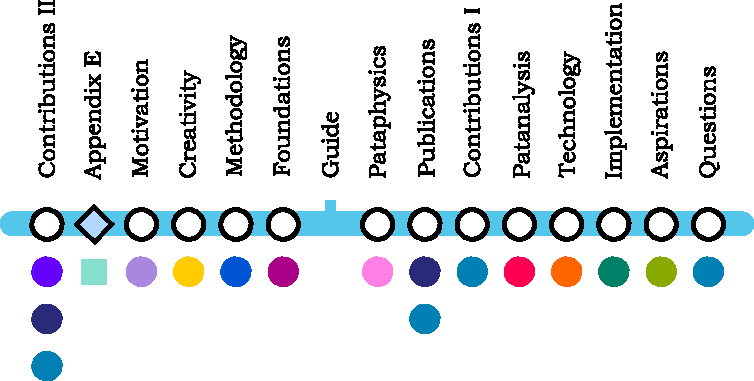
\includegraphics{intro.pdf}
\end{figure}

\vfill

{\sffamily 

The first chapter serves as an introduction to the thesis and as such leads into the most important topics (pataphysics \pata, creativity \creat, technology \tech, evaluation \eval) and their interplay (see foundations \found, interpretation \inter) which resulted in the artefact \url{pata.physics.wtf} \imple. The concept of \acf{AMC} is explained and the main original contributions to knowledge are highlighted. More on the pataphysical algorithms (`Contributions I') can be found in chapter~\ref{ch:pataphysics} \pata~ (for literary context of the concepts which inspired the algorithms), \ref{ch:technology} \tech~ (for technical background information) and~\ref{ch:implementation} \imple~ (for detailed technical descriptions of the algorithms and how they were incorporated into the creative search tool \url{pata.physics.wtf}). More details about the evaluation/interpretation framework (`Contributions II'---including the subjective criteria and objective constraints) can be found in chapter~\ref{ch:interpretation} \inter. The transdisciplinary methodology employed in this project is described in chapter~\ref{ch:methodology} \metho, and the key inspirations (Jarry, Borges, Queneau) and others are elaborated in chapter~\ref{ch:insporations} \inspi. The \nameref{ch:analysis} chapter \anal~ goes into an analysis of the various theoretical and practical aspects of this thesis. Appendix~\ref{app:pub} \appe~ shows copies of all published papers in full. These are also summarised in the \nameref{ch:applications} chapter--section~\ref{s:public} \appli. Any future work is discussed in chapter~\ref{ch:future} \aspi~ and the conclusion chapter (§~\ref{ch:outroduction}) \outro~ provides answers to the research questions introduced here.
}

\begin{figure}[!htbp]
\centering
  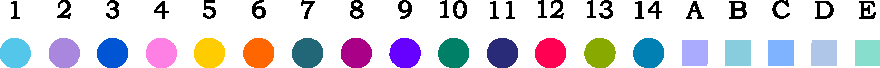
\includegraphics[width=\textwidth]{legend.pdf}
\end{figure}



\newpage
\section{From the Inspirations to Paris by Sea}

\vspace{1cm}
\begin{figure}[!htbp]
\centering
  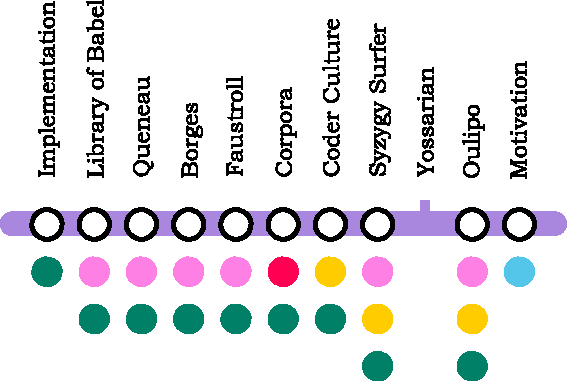
\includegraphics{inspi.pdf}
\end{figure}

\vfill

{\sffamily 

The inspirations referenced in this chapter have influenced many aspects of this project. The Syzygy Surfer by Hendler and Hugill \autocite*{Hendler2011, Hendler2013} for instance forms the basis for all of the research covered in this thesis and is also mentioned in chapter~\ref{ch:creativity} \creat, \ref{ch:pataphysics} \pata, and \ref{ch:implementation} \imple. The \ac{oulipo} is also covered in these chapters. These influences in general have already been introduced in the \nameref{ch:introduction} \intro. Faustroll's `library of equivalent books' in Jarry's novel ``The Exploits and Opinions of Dr. Faustroll, Pataphysician'' \autocite*{Jarry1996} forms a key element in two main features of \url{pata.physics.wtf}, namely one of the two corpora (the other one being the Shakespeare corpus) introduced in section~\ref{s:corpora} \imple~ and the base text used in the clinamen algorithm (see section~\ref{s:clinamenalgo}) \imple. The literary context for the novel, the character and library are discussed in chapter~\ref{ch:pataphysics} \pata. The two corpora mentioned above are also further covered in the \nameref{ch:analysis} chapter \anal, for example: comparing the search results produced by the two different corpora (see tables~\ref{tab:faustshake} and \ref{tab:algonums} and also section~\ref{s:analindex}), and changing the base text in the clinamen algorithm (section~\ref{s:basetext}).
}

\begin{figure}[!htbp]
\centering
  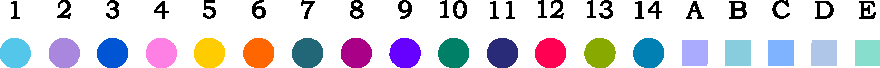
\includegraphics[width=\textwidth]{legend.pdf}
\end{figure}


\newpage

\section{From Pataphysics to Paris by Sea}

\begin{figure}[!htb]
\centering
  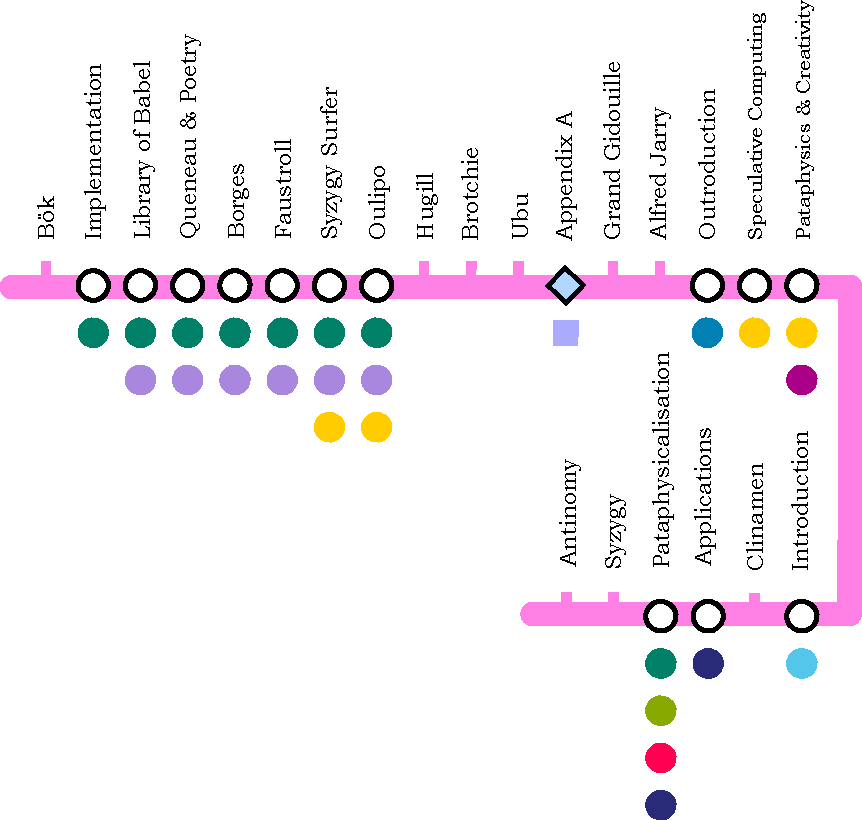
\includegraphics{pata.pdf}
\end{figure}

{\sffamily 
A lot of what is covered in this chapter is used in the \nameref{ch:implementation} \imple~ and \nameref{ch:inspirations} \inspi~ chapters. Some of it also relates to chapter~\ref{ch:creativity} \creat, such as the \ac{OULIPO}. This chapter contains descriptions for each of the pataphysical concepts used to inspire the algorithms for \url{pata.physics.wtf} (clinamen §~\ref{s:clinamen}, syzygy §~\ref{s:syzygy} and antinomy §~\ref{s:antinomy}). This is part of the pataphysicalisation process described in section~\ref{s:algorithms} \imple. Possible adaptations to this process are described in chapter~\ref{ch:future} \aspi, a thorough analysis of the algorithms is conducted in chapter~\ref{ch:analysis} anal (specifically section~\ref{s:pataphyanalysis}), and details on how they have been used by others (Dennis \autocite*{Dennis2016} and Hugill et al. \autocite*{Hugill2014a}) are given in chapter~\ref{ch:applications} \appli. Appendix~\ref{app:random} \appa~ includes a list of Jarry's written work. 
}

\begin{figure}[!htb]
\centering
  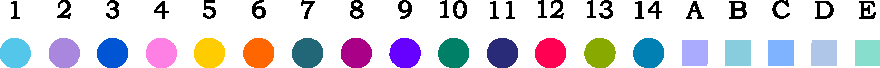
\includegraphics[width=\textwidth]{legend.pdf}
\end{figure}

\stopcontents[chapters]

\end{document}
